% Options for packages loaded elsewhere
\PassOptionsToPackage{unicode}{hyperref}
\PassOptionsToPackage{hyphens}{url}
\documentclass[
]{ltjsarticle}
\usepackage{xcolor}
\usepackage[margin=20mm]{geometry}
\usepackage{amsmath,amssymb}
\setcounter{secnumdepth}{-\maxdimen} % remove section numbering
\usepackage{iftex}
\ifPDFTeX
  \usepackage[T1]{fontenc}
  \usepackage[utf8]{inputenc}
  \usepackage{textcomp} % provide euro and other symbols
\else % if luatex or xetex
  \usepackage{unicode-math} % this also loads fontspec
  \defaultfontfeatures{Scale=MatchLowercase}
  \defaultfontfeatures[\rmfamily]{Ligatures=TeX,Scale=1}
\fi
\usepackage{lmodern}
\ifPDFTeX\else
  % xetex/luatex font selection
\fi
% Use upquote if available, for straight quotes in verbatim environments
\IfFileExists{upquote.sty}{\usepackage{upquote}}{}
\IfFileExists{microtype.sty}{% use microtype if available
  \usepackage[]{microtype}
  \UseMicrotypeSet[protrusion]{basicmath} % disable protrusion for tt fonts
}{}
\makeatletter
\@ifundefined{KOMAClassName}{% if non-KOMA class
  \IfFileExists{parskip.sty}{%
    \usepackage{parskip}
  }{% else
    \setlength{\parindent}{0pt}
    \setlength{\parskip}{6pt plus 2pt minus 1pt}}
}{% if KOMA class
  \KOMAoptions{parskip=half}}
\makeatother
\usepackage{graphicx}
\makeatletter
\newsavebox\pandoc@box
\newcommand*\pandocbounded[1]{% scales image to fit in text height/width
  \sbox\pandoc@box{#1}%
  \Gscale@div\@tempa{\textheight}{\dimexpr\ht\pandoc@box+\dp\pandoc@box\relax}%
  \Gscale@div\@tempb{\linewidth}{\wd\pandoc@box}%
  \ifdim\@tempb\p@<\@tempa\p@\let\@tempa\@tempb\fi% select the smaller of both
  \ifdim\@tempa\p@<\p@\scalebox{\@tempa}{\usebox\pandoc@box}%
  \else\usebox{\pandoc@box}%
  \fi%
}
% Set default figure placement to htbp
\def\fps@figure{htbp}
\makeatother
\setlength{\emergencystretch}{3em} % prevent overfull lines
\providecommand{\tightlist}{%
  \setlength{\itemsep}{0pt}\setlength{\parskip}{0pt}}
\usepackage{bookmark}
\IfFileExists{xurl.sty}{\usepackage{xurl}}{} % add URL line breaks if available
\urlstyle{same}
\hypersetup{
  hidelinks,
  pdfcreator={LaTeX via pandoc}}

\author{}
\date{}

\begin{document}

\section{Waveform Invariance and a Contrast Law for the Two-Copy
Common-Relative-Phase Superposition of a Half-Wavelength Odd-Harmonic
Isolated Peak
Wave}\label{waveform-invariance-and-a-contrast-law-for-the-two-copy-common-relative-phase-superposition-of-a-half-wavelength-odd-harmonic-isolated-peak-wave}

\textbf{Subtitle}: Giving two copies a common relative phase leaves the
waveform unchanged and scales the squared amplitude by the square of the
cosine of the relative phase

\textbf{Author}: Noriaki Kihara\\
\textbf{Version}: v0.1\\
\textbf{Date}: 2026-06-26\\
\textbf{DOI}: Version 10.5281/zenodo.20923462 (this version) / Concept
10.5281/zenodo.20923461 (cite this; always resolves to the latest
version)\\
\textbf{Zenodo}: https://zenodo.org/records/20923462\\
\textbf{Position}: First draft as an observational and organizing paper.
For the isolated peak wave formed by superposing constant-amplitude odd
harmonics on a half-wavelength phase interval, it records, as an
elementary property of Fourier sums and trigonometric identities, that
giving two copies a common relative phase leaves the waveform (shape,
the zeros at both ends, the localization width) independent of that
relative phase, while only the squared amplitude changes in proportion
to the square of the cosine of the relative phase. It does not derive
physical laws, assert observational facts, or give any particular
physical interpretation.

\begin{center}\rule{0.5\linewidth}{0.5pt}\end{center}

\subsection{Abstract}\label{abstract}

On the half-wavelength phase interval \(\varphi\in[-\pi/2,\pi/2]\), the
wave formed by superposing constant-amplitude odd harmonics,

\[
S_N(\varphi)=\sum_{m=0}^{(N-1)/2}\cos\!\big((2m+1)\varphi\big),
\]

is an isolated peak wave with a peak at the center and zeros at both
ends (\(N\) is the highest odd-harmonic order, \(N\) odd).

This paper observes the wave obtained by giving two copies of this wave
a common relative phase \(2\alpha\) applied identically to all
harmonics,

\[
\psi_\alpha(\varphi)=\sum_{m=0}^{(N-1)/2}\Big[\cos\!\big((2m+1)\varphi-\alpha\big)+\cos\!\big((2m+1)\varphi+\alpha\big)\Big].
\]

A trigonometric identity immediately gives
\(\psi_\alpha(\varphi)=2\cos\alpha\cdot S_N(\varphi)\), so the squared
amplitude is \(I_\alpha(\varphi)=4\cos^2\!\alpha\cdot S_N(\varphi)^2\).
This means: (i) \textbf{the waveform does not depend on the relative
phase \(\alpha\)} (the normalized waveform coincides with that of a
single copy); (ii) \textbf{the relative phase appears only as an overall
cosine-squared contrast factor \(\cos^2\!\alpha\) on the squared
amplitude}. This paper records the property only as an observation about
Fourier sums and a trigonometric identity, and gives no physical
interpretation.

\begin{center}\rule{0.5\linewidth}{0.5pt}\end{center}

\subsection{1. Introduction}\label{introduction}

Superposing constant-amplitude odd harmonics only, on a half-wavelength
interval, forms an isolated peak wave with a dominant main peak at the
center and zeros at both ends. This paper observes not the properties of
that isolated peak wave itself, but how the waveform and the squared
amplitude behave \textbf{when two copies of it are superposed under a
common relative phase}.

The relative phase treated here is a constant offset \(\pm\alpha\) added
\textbf{in common} to the phase of every harmonic. That is, it is not a
quantity that shifts the phase in proportion to the harmonic order
\(n=2m+1\) (which would amount to a translation within the interval),
but a phase quantity imposed identically on all harmonics. This
distinction is a premise of the present observation and is made explicit
in §2.

Notation and formulas follow a standard analysis text {[}1{]}. The main
result (§3) is an elementary fact obtained merely by applying the
product-to-sum identity
\(\cos(u-\alpha)+\cos(u+\alpha)=2\cos u\cos\alpha\) to each harmonic.

\begin{center}\rule{0.5\linewidth}{0.5pt}\end{center}

\subsection{2. Definitions}\label{definitions}

\subsubsection{2.1 Isolated peak wave}\label{isolated-peak-wave}

For the variable \(\varphi\in[-\pi/2,\pi/2]\), define the
constant-amplitude odd-harmonic sum

\[
S_N(\varphi)=\sum_{m=0}^{(N-1)/2}\cos\!\big((2m+1)\varphi\big)
\tag{2.1}
\]

where \(N\) is the highest odd-harmonic order, \(N\) odd, and the sum
contains the \((N+1)/2\) terms \(1,3,5,\dots,N\). The wave \(S_N\) has a
main peak at the center \(\varphi=0\),

\[
S_N(0)=\frac{N+1}{2},
\tag{2.2}
\]

and vanishes at both ends \(\varphi=\pm\pi/2\). The latter holds because
each odd harmonic satisfies \(\cos\!\big((2m+1)(\pm\pi/2)\big)=0\),
independently of the value of \(S_N\) or the number of terms. As a
non-negative observable we use the squared amplitude

\[
I_N(\varphi)=\big|S_N(\varphi)\big|^2=S_N(\varphi)^2.
\tag{2.3}
\]

Figure 1 shows each odd harmonic (\(n=1,3,5,7,9\), i.e.~\(N=9\)) and
their coherent sum (black) over the central region of the
half-wavelength closed interval \(\pm 90^\circ\ (=\pm\pi/2)\). One sees
that the sum becomes an isolated peak wave with a main peak at the
center.

\begin{figure}
\centering
\pandocbounded{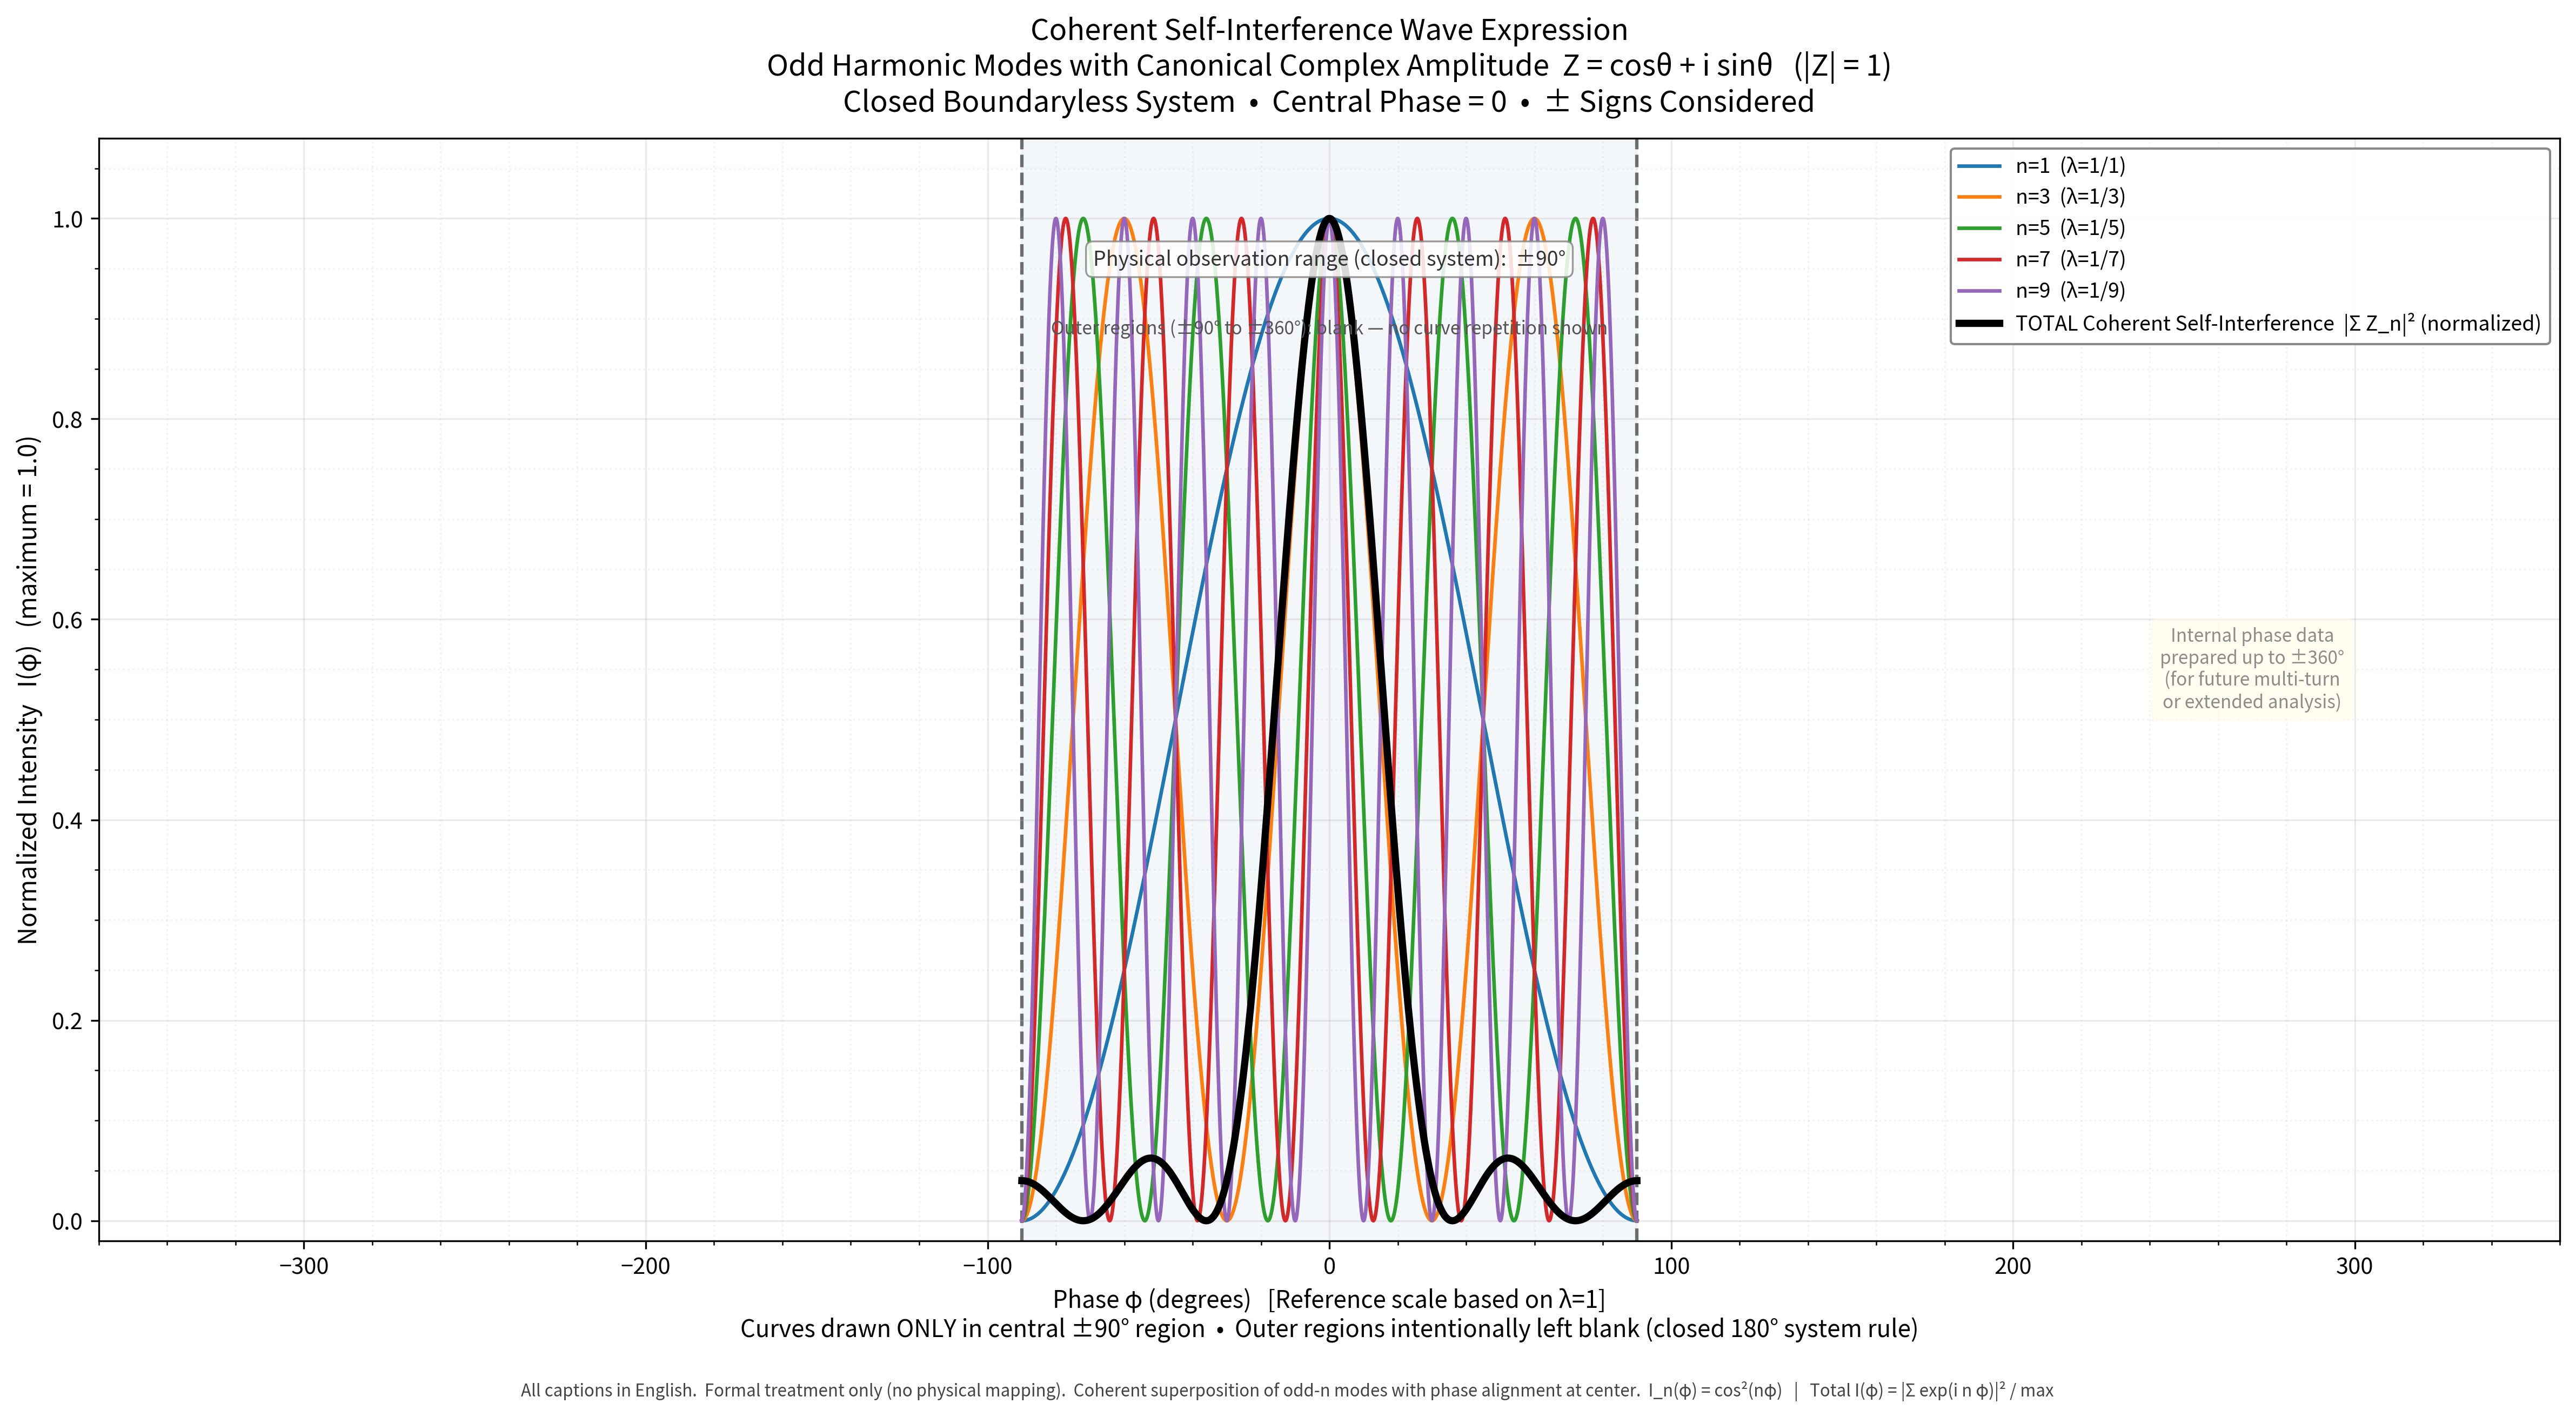
\includegraphics[keepaspectratio,alt={Figure 1}]{coherent_self_interference_odd_modes.png}}
\caption{Figure 1}
\end{figure}

\textbf{Figure 1}: Constant-amplitude odd harmonics (\(n=1,3,5,7,9\),
canonical complex amplitude \(Z=\cos\theta+i\sin\theta\), \(|Z|=1\)) and
their coherent sum (black), drawn normalized over the central region of
the half-wavelength closed interval \(\pm 90^\circ\).

\subsubsection{2.2 Two-copy superposition under a common relative
phase}\label{two-copy-superposition-under-a-common-relative-phase}

Define the wave obtained by giving two copies of \(S_N\) a common
relative phase \(\pm\alpha\) applied to all harmonics,

\[
\psi_\alpha(\varphi)
=\sum_{m=0}^{(N-1)/2}\Big[\cos\!\big((2m+1)\varphi-\alpha\big)+\cos\!\big((2m+1)\varphi+\alpha\big)\Big].
\tag{2.4}
\]

Here \(\alpha\) is a constant independent of the harmonic order
\(n=2m+1\), and the relative phase difference of the two copies is
uniformly \(2\alpha\) for all harmonics. The observable is the squared
amplitude

\[
I_\alpha(\varphi)=\big|\psi_\alpha(\varphi)\big|^2=\psi_\alpha(\varphi)^2.
\tag{2.5}
\]

\begin{center}\rule{0.5\linewidth}{0.5pt}\end{center}

\subsection{3. Observation: waveform invariance and a contrast
law}\label{observation-waveform-invariance-and-a-contrast-law}

\subsubsection{3.1 Identity}\label{identity}

Applying the product-to-sum identity

\[
\cos\!\big(n\varphi-\alpha\big)+\cos\!\big(n\varphi+\alpha\big)=2\cos\!\big(n\varphi\big)\cos\alpha
\tag{3.1}
\]

to each harmonic \(n=2m+1\) in Eq. (2.4), and noting that \(\cos\alpha\)
is a common factor independent of \(n\) and so comes out of the sum,

\[
\psi_\alpha(\varphi)
=2\cos\alpha\sum_{m=0}^{(N-1)/2}\cos\!\big((2m+1)\varphi\big)
=2\cos\alpha\cdot S_N(\varphi).
\tag{3.2}
\]

This is an exact identity, not an approximation.

\subsubsection{3.2 Squared amplitude, invariance, and
contrast}\label{squared-amplitude-invariance-and-contrast}

Squaring Eq. (3.2),

\[
I_\alpha(\varphi)=4\cos^2\!\alpha\cdot S_N(\varphi)^2=4\cos^2\!\alpha\cdot I_N(\varphi).
\tag{3.3}
\]

Two consequences follow immediately.

\textbf{(1) Waveform invariance.} All dependence on \(\varphi\) resides
in \(S_N(\varphi)^2=I_N(\varphi)\), and the relative phase \(\alpha\)
appears only in the prefactor \(4\cos^2\!\alpha\). Hence the waveform
normalized by its main-peak value,

\[
\widehat{I}_\alpha(\varphi):=\frac{I_\alpha(\varphi)}{I_\alpha(0)}
=\frac{4\cos^2\!\alpha\,I_N(\varphi)}{4\cos^2\!\alpha\,I_N(0)}
=\frac{I_N(\varphi)}{I_N(0)}=\widehat{I}_N(\varphi),
\tag{3.4}
\]

does not depend on \(\alpha\) and coincides exactly with the normalized
waveform \(\widehat{I}_N\) of a single copy (for \(\cos\alpha\neq0\)).
The shape, the zeros at both ends \(\varphi=\pm\pi/2\), and the
localization width near the main peak are all invariant under a change
of the relative phase.

\textbf{(2) Contrast law.} The unnormalized peak squared amplitude is

\[
I_\alpha(0)=4\cos^2\!\alpha\cdot I_N(0)=(N+1)^2\cos^2\!\alpha
\tag{3.5}
\]

(using Eq. (2.2)), and relative to the in-phase value \((N+1)^2\) at
\(\alpha=0\),

\[
\frac{I_\alpha(0)}{I_0(0)}=\cos^2\!\alpha.
\tag{3.6}
\]

That is, the relative phase \(2\alpha\) scales the overall squared
amplitude by \(\cos^2\!\alpha\) without changing the waveform: maximal
at \(\alpha=0\) (relative phase \(0\)) and zero at \(\alpha=\pi/2\)
(relative phase \(\pi\)).

As a concrete example, for the same \(N=9\) (\(n=1,3,5,7,9\)) and
\(\alpha=15^\circ\) (relative phase \(30^\circ\)) as in Figures 1 and 2,
one has \(I_0(0)=(N+1)^2=100\),
\(I_\alpha(0)=100\cos^2 15^\circ\approx 93.30\), and the contrast factor
\(\cos^2 15^\circ\approx 0.9330\).

\subsubsection{3.3 Confirmation by figure}\label{confirmation-by-figure}

Figure 2 shows the two-copy superposition \(I_\alpha\) for \(N=9\) and
\(\alpha=15^\circ\) (relative phase \(30^\circ\)), normalized by its
main-peak value, over the full range \(\pm 360^\circ\). As Eq. (3.4)
states, this normalized waveform coincides with the normalized waveform
of a single copy (the square of the black curve of Figure 1). The only
change due to the relative phase is the contrast factor
\(\cos^2\!\alpha\), which is divided out by normalization and therefore
does not appear in a normalized plot. This figure thus displays the
consequence of Eq. (3.3) --- ``the relative phase changes only the
amplitude, not the waveform'' --- as the invariance of the normalized
waveform.

\begin{figure}
\centering
\pandocbounded{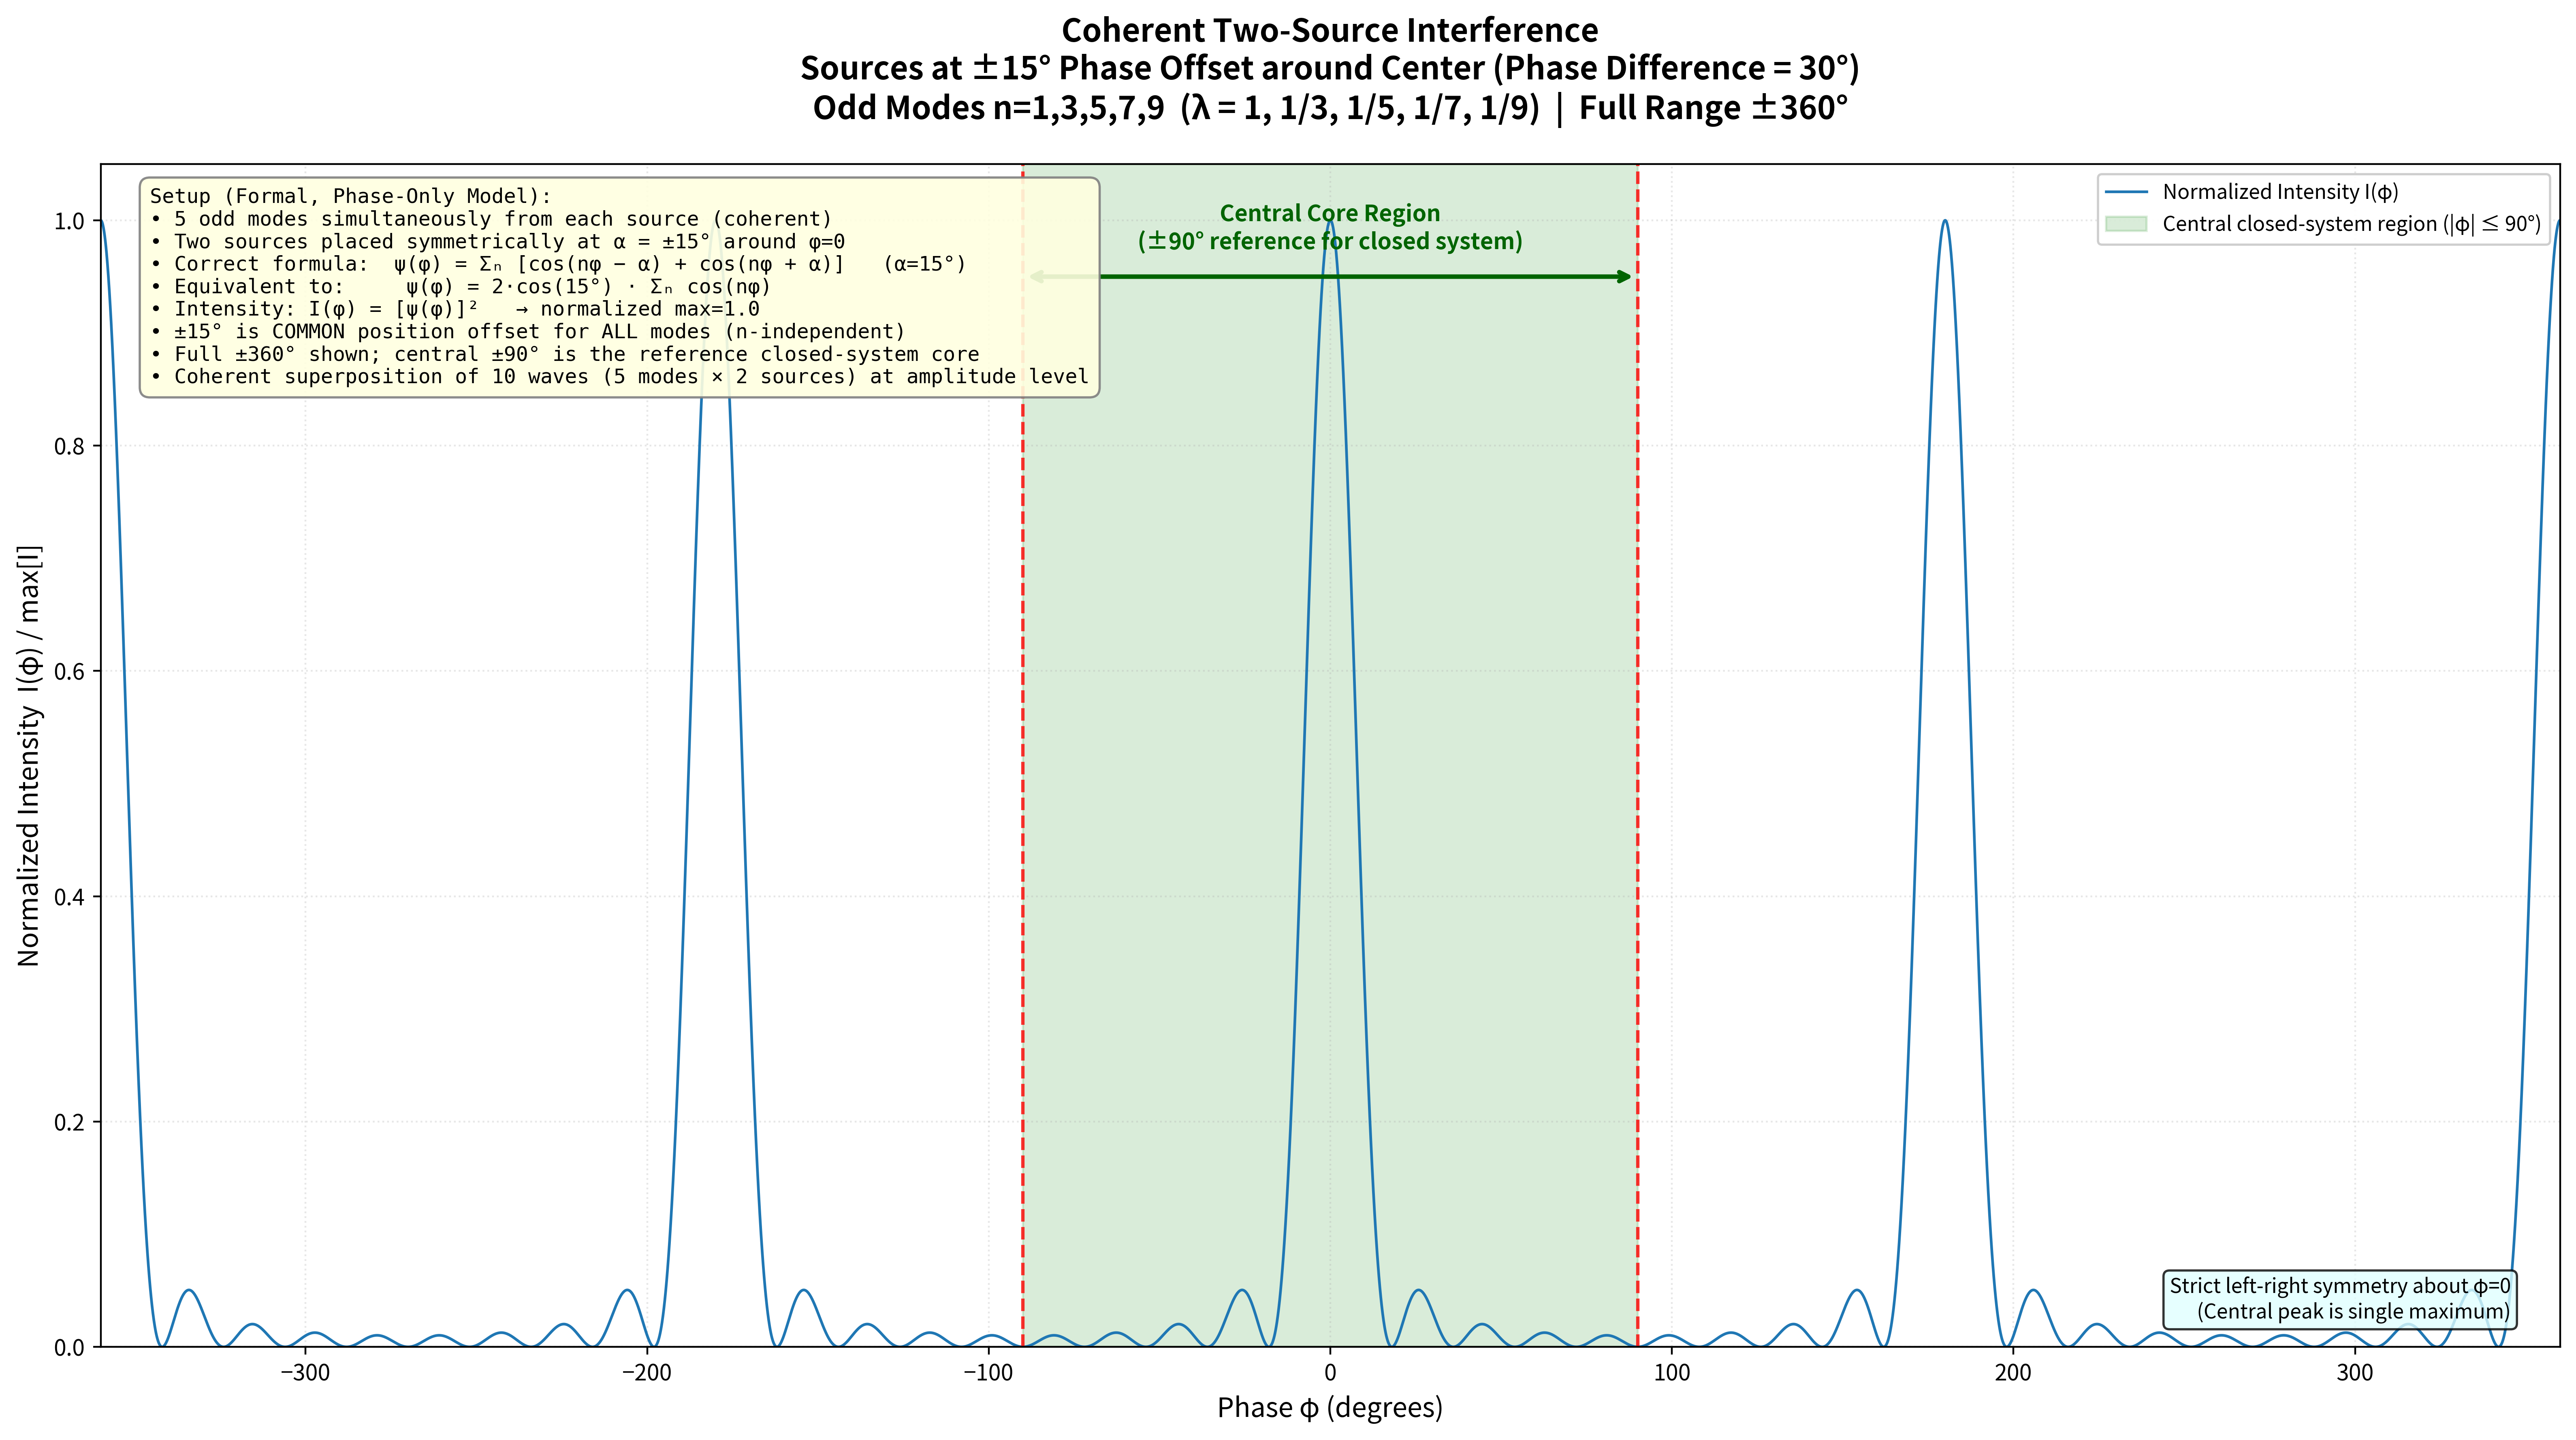
\includegraphics[keepaspectratio,alt={Figure 2}]{two_source_coherent_interference_corrected_v4_hires.png}}
\caption{Figure 2}
\end{figure}

\textbf{Figure 2}: Normalized squared amplitude of the two-copy
superposition \(I_\alpha\) (\(N=9\), relative phase
\(2\alpha=30^\circ\), i.e.~\(\alpha=15^\circ\)). Full range
\(\pm 360^\circ\), with the central \(\pm 90^\circ\ (=\pm\pi/2)\)
highlighted. The normalized waveform coincides with that of a single
copy (waveform invariance).

\begin{center}\rule{0.5\linewidth}{0.5pt}\end{center}

\subsection{4. Conclusion}\label{conclusion}

For the wave
\(\psi_\alpha=\sum[\cos(n\varphi-\alpha)+\cos(n\varphi+\alpha)]\)
obtained by giving two copies of the constant-amplitude odd-harmonic sum
\(S_N\) on the half-wavelength phase interval
\(\varphi\in[-\pi/2,\pi/2]\) a common relative phase \(\pm\alpha\), the
product-to-sum identity yields

\[
\psi_\alpha(\varphi)=2\cos\alpha\cdot S_N(\varphi),
\qquad
I_\alpha(\varphi)=4\cos^2\!\alpha\cdot I_N(\varphi).
\]

From this exact identity the following results follow.

\textbf{(1) Waveform invariance}

\begin{itemize}
\tightlist
\item
  The normalized waveform \(\widehat{I}_\alpha=\widehat{I}_N\) does not
  depend on the relative phase \(\alpha\). The shape, the zeros at both
  ends, and the localization width near the main peak are invariant
  under a change of the relative phase.
\end{itemize}

\textbf{(2) Contrast law}

\begin{itemize}
\tightlist
\item
  The relative phase \(2\alpha\) scales the squared amplitude by
  \(\cos^2\!\alpha\) without changing the waveform (Eq. (3.6)): maximal
  at \(\alpha=0\) and zero at \(\alpha=\pi/2\).
\end{itemize}

All of the above are elementary facts obtained merely by applying the
product-to-sum identity
\(\cos(n\varphi-\alpha)+\cos(n\varphi+\alpha)=2\cos(n\varphi)\cos\alpha\)
to a constant-amplitude odd-harmonic sum, and no physical interpretation
is given.

\begin{center}\rule{0.5\linewidth}{0.5pt}\end{center}

\subsection{References}\label{references}

{[}1{]} T. Takagi, \emph{Kaiseki Gairon} (Introduction to Analysis), 3rd
revised ed., Iwanami Shoten, 1961 (chapter on Fourier series:
trigonometric series, closed forms of cosine sums, product-to-sum
formulas).

\end{document}
